\chapter{The Bow Model}

A scientific model is a simplification and abstraction of reality, often formulated in a mathematical way.
A good model reduces the complexity of a real system by including only its most significant aspects and disregarding less significant ones.
The results of analyzing this simplified model can then be used to draw conclusions about the real system.

What aspects of reality a model has to reflect depends on the kinds of questions it seeks to answer.
The first step for developing a bow model is therefore to clarify its scope and intended application.

\section{Scope of the Model}
\label{section:model-scope}

In the case of VirtualBow the purpose of the bow model is to give users the ability to evaluate the bow designs they come up with.
So what characteristics make a bow design a good one and what are their implications for the bow model?
Many things come to mind, but we limit ourselves to the following three categories:

\begin{enumerate}
\item \textbf{Viability}: Can the design be realised? Do the materials withstand the arising loads when the bow is being used?
To be able to judge this the model has to accurately predict the distribution of stress across the limbs as well as the tensile forces in the string that arise when drawing and shooting the bow.

\item \textbf{Performance}: Important performance characteristics are the arrow's velocity, kinetic energy and the bow's degree of efficiency, i.e. the percentage of the stored elastic energy that is converted into kinetic energy of the arrow during the shot.
To capture these things the model has to reflect all major mechanisms of efficiency loss in a bow.
We will later see what those are when we look at scientific research.

\item \textbf{Comfort}: Viability and raw performance aren't everything.
A bow design will also be judged by it's influence on the archer, like the draw force, the shape of the draw curve (no "stacking", i.e. increasing stiffness towards the end of draw) and the dynamic forces exerted to the shooter ("hand shock").
\end{enumerate}

Any physical effects in archery that don't (significantly) affect one of those categories above are outside the scope of VirtualBow and the bow model doesn't need to include them.
Exterior ballistics is an example for this, another one is the bending motion of the arrow (Archer's Paradox).

Now the next question is: How does a bow model have to look like in order to capture the things listed above?
That's not easy to answer, but luckily there has been done quite some scientific research about bow and arrow physics in the past, so we don't have to start completely from scratch.
The next section therefore examines some of that research before we define our own model.

\section{Literature Review}

Research about the mechanics of bow and arrow goes back to at least the 1930s, when C.N.~Hickman, P.E.~Klopstek and others performed systematic experiments and developed simple mathematical models.
Without modern computers available these early models were still limited in their complexity by what could be solved analytically.
The focus was therefore more on qualitative insight rather than accurate prediction.
One of those early models is the~\textit{Hickman Model}~\cite{bib:hi37}, published in~1937.
It assumes two rigid limbs that are connected to the stationary rest of the bow via elastic hinges as shown in figure~\ref{fig:model:hickman}.
Even though this is a huge simplification, this model can already be used to investigate the efficiency of a bow, i.e. how it transfers its stored elastic energy to an arrow.

\begin{figure}[h]
\centering
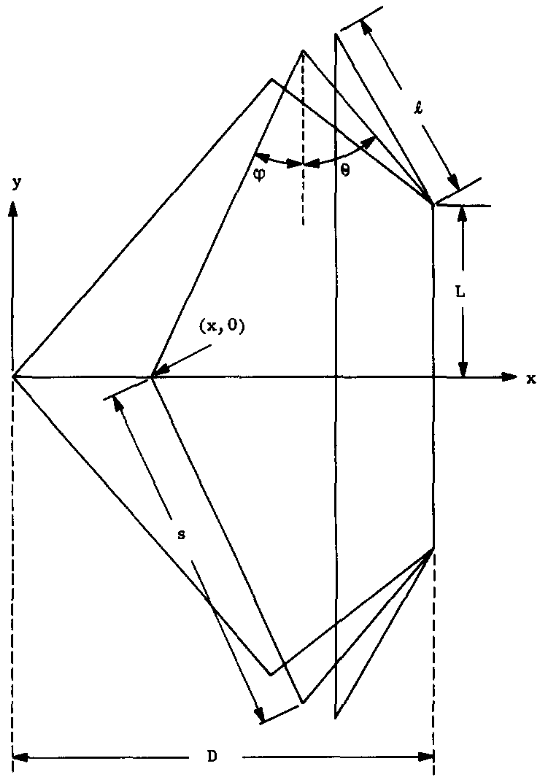
\includegraphics[width=0.4\textwidth]{figures/model/hickman}
\caption{Hickman model as used by W.C. Marlow \cite{bib:ma80}}
\label{fig:model:hickman}
\end{figure}

An important modification to the Hickman model was suggested by W.C.~Marlow in 1980~\cite{bib:ma80}.
It was already well-known that the original Hickman model with an inextensible string severely overpredicted a bow's degree of efficiency.
(Predicted efficiencies typically over 90\% while measurements suggest values between 70\% and 85\% for most bows.)
Popular explanations for this discrepancy were effects like hysteresis and air resistance.
Marlow however found another reason: With an inextensible string (as in Hickman's original model) the arrow exits the bow exactly at brace height, where the limbs have zero velocity.
Only the kinetic energy of the string remains in the bow, the rest is transferred to the arrow.
Marlow then showed that accounting for the elasticity of the string shifts the point of exit for the arrow away from the braced position, such that the limbs still have substantial kinetic energy left. In his numerical example the modification reduces the predicted efficiency to~78\% as opposed to~92\% previously.
Of the energy remaining in the bow,~11\% were the kinetic energy of the limbs,~9\% the kinetic energy of the string and~2\% the potential energy of limbs and string.

This leads to an important realization: The efficiency of a bow is mainly determined by the kinetic energy that stays in the system due to mass and elasticity of the string and the mass distribution of the limbs. The contribution of dissipative effects like air resistance and hysteresis to the overall efficiency was estimated by Marlow to be less than~2\% and~3\% respectively.

The widespread availability of digital computers eventually made it possible to simulate much more detailed models and therefore make more accurate predictions.
Much notable work in this area has been done by Dr.~Bob~Kooi and his co-authors.
Over the course of the~1980s and~90s they published a good amount of papers about the mechanics of bow and arrow in which they utilize numerical methods to solve increasingly complex mathematical models.

The first one of those papers is titled \textit{On the static deformation of a bow}~\cite{bib:kosp80} and investigates the storage of deformation energy in bows with and without recurve. Figure~\ref{fig:model:kooi} shows the model used there.
The bow is assumed to be symmetric and has an inextensible string.
The limbs are represented by an Euler-Bernoulli beam, which is an infinitely thin, elastic line with a certain (varying) bending stiffness for which the Euler-Bernoulli assumptions hold.
These are assumptions about the kinematics of the deformation, namely that the cross sections of the beam always stay flat and perpendicular to its centerline. This is typically a good approximation for slender beams, that is beams whose length is much larger than their cross section dimensions. Kooi uses the general version of the Euler-Bernoulli equation that accounts for arbitrarily large deformation. Combining this with geometric constraints for the string and some boundary conditions leads to the bow's equations of equilibrium, a free-boundary value problem for a set of ordinary differential equations. The equations of equilibrium are solved numerically for specific draw lengths of the bow.

\begin{figure}[h]
\centering
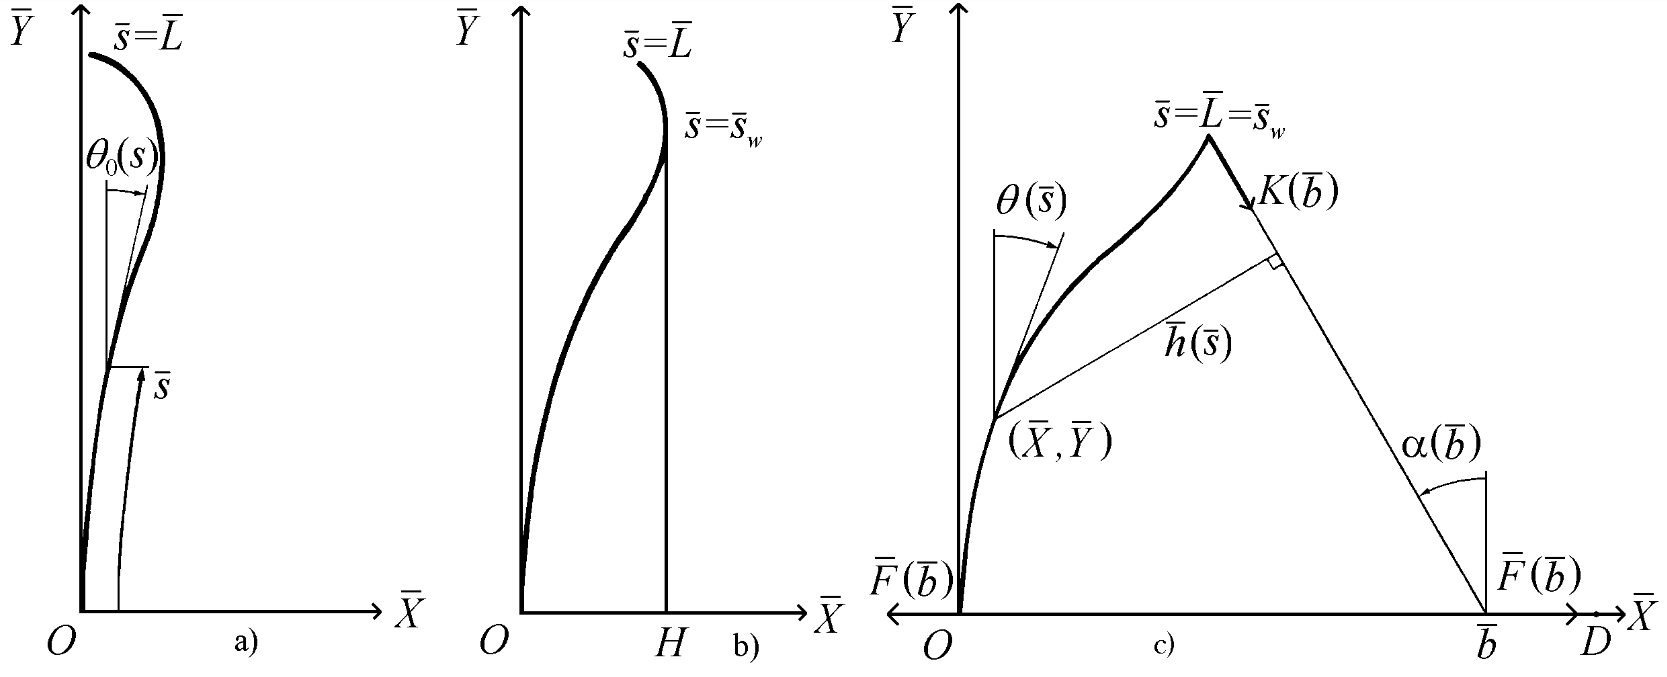
\includegraphics[width=0.8\textwidth]{figures/model/kooi}
\caption{Bow model used by Bob Kooi \cite{bib:kosp80}}
\label{fig:model:kooi}
\end{figure}

In subsequent papers titled \textit{On the mechanics of the bow and arrow}~\cite{bib:kooi81} and \textit{On the mechanics of the modern working-recurve bow}~\cite{bib:kooi91} Kooi also considers the dynamic case. Like Marlow he uses a linear-elastic string and assumes the arrow as a concentrated point mass. The equations of motion for the system form a moving-boundary value problem for a set of partial differential equations. They are solved numerically by using a finite-difference method with complete discretization. (Both space and time are approximated by a discrete "grid" of values. The partial derivatives in the governing equations are then approximated by finite difference quotients operating on those grid values. The resulting large number of difference equations can then be solved with a computer program.)

In the paper \textit{On the Mechanics of the Arrow: Archer's Paradox}~\cite{bib:kosp97}, Kooi refines his model even more by including an elastic arrow with a sliding contact to the bow's grip. This makes it possible to analyze the Archer's Paradox: The phenomenon of arrows going around the grip of a bow by performing a bending motion in the horizontal plane. The dynamics of the arrow are however treated partly decoupled from the bow's dynamics: Only the influence of the bow on the arrow's motion is considered, the other way around is neglected. This is in line with our assumption from section~\ref{section:model-scope} that the bending motion of the arrow doesn't contribute much to a bow's overall performance and is therefore out of scope for our model.

\section{Model Definition}

We have now learned enough in order to define our own bow model. First of all a few words on the general modeling approach. As we saw in the previous section, any decently complex bow model cannot be solved analytically but has to be combined with some sort of numerical method for calculating an approximate solution. Models based on continuum mechanics (e.g. Euler-Bernoulli beam theory) always have an infinite number of degrees of freedom and will eventually have to be approximated by a discrete system with finitely many degrees of freedom in order to be solvable by a computer program. This step is called discretization. Kooi for example, like a true mathematician, formulates the complete equations of motion for his continuous bow model and only then starts to employ a discretization technique (in this case a finite difference method) to solve those equations. This results in a clear separation between the mathematical model and the numerical solution methods.

We're going to use more of an engineering approach here instead and start with a discrete system in the first place. We do this by constructing the continuous parts of the bow from a large number of so-called finite elements. A finite element is an approximation of a little part of a continuous structure, e.g. a beam or a bar, but with only finitely many degrees of freedom, namely the displacements of the nodes at which the elements are connected to each other. The more elements are used, the better the approximation gets and the closer the results will be to the exact solution.

The finite element method leads to a (potentially large) system of ordinary differential equations as the equations of motion, which can be solved by standard numerical methods as we will see later.

\begin{figure}[h]
\centering
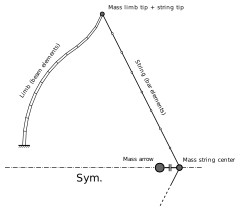
\includegraphics[width=0.8\textwidth]{figures/model/bow-simulator}
\caption{Finite element model of the bow}
\label{fig:model:bow-simulator}
\end{figure}

Figure~\ref{fig:model:bow-simulator} shows the finite element approximation of our bow model. Like Kooi's model it is symmetric with respect to the horizontal plane, assumes the limbs to satisfy the Euler-Bernoulli assumptions and neglects any dissipative effects like air resistance and hysteresis. The limbs are therefore made up of Euler-Bernoulli beam elements. A concentrated point mass is placed at the tips to account for any added weight, like overlays for example.

The string, as opposed to the limbs, only transfers longitudinal forces and is therefore approximated by linear-elastic bar elements. We limit ourselves to linear elasticity for pragmatic reasons: Obtaining the exact nonlinear stress-strain curve of a particular string material is pretty difficult. Instead, any material nonlinearity (which can be the case especially for modern synthetic materials) will have to be accounted for by using an "average" stiffness. In the previous section we saw that the mass properties of the string are fairly important, so in addition to the mass of the string itself there are two additional point masses at the tips and center to account for things like servings, nocking point, etc.

The arrow is another point mass, as already justified earlier. It is connected to the string by an ideal, frictionless contact without any release force. This means that the arrow will be released as soon as the string doesn't push against/accelerate it anymore.

Not shown in figure~\ref{fig:model:bow-simulator} are the contact elements that prevent the string nodes from passing through the limb, thereby making it possible to simulate recurves. These are also ideal contacts without any friction.

All in all, there are four different types of elements needed:

\begin{itemize}
\item Beam Elements (Limbs)
\item Bar Elements (String)
\item Mass Elements (Arrow + additional masses)
\item Contact Elements (String to limb contact)
\end{itemize}

All of them have to account for arbitrarily large displacements and are therefore geometrically nonlinear (even though all the materials are linear-elastic).

In the next chapters we will first show how the equations of motion for a finite element system can be assembled from the equations of motion for the single elements. We will then derive the equations of motion for the element types listed above. Finally we're going to discuss the numerical solution of those equations for the static and dynamic case and how this is implemented in VirtualBow.

\newpage
\section{Limb Geometry}

\subsection{Profile Curve}

A section of the profile curve is to be determined by two control points $\{ s_0,\,\varphi_0,\,x_0,\,y_0 \}$ and $\{ s_1,\,\varphi_1,\,x_1,\,y_1 \}$, with $s$ beinig the arc length along the curve, $\varphi$ being the angle between the curve's tangent and the x-axis and $x$ and $y$ being the position of the point.
The second/end point might be incompletely specified by omitting up to two values.

We choose the curvature of our section to vary quadratically on the arc length, which will give the resulting curve the needed degrees of freedom to exactly match the end point if completely specified.
%
\begin{equation}
\kappa(s) = c_0 + c_1\,s + c_2\,s^2,\quad s \in [0,\,c_3]
\end{equation}
%
This description of the curvature includes lines, circles and Euler Spirals as special cases.
The angle and coordinates of the curve can be calculated by integration,
%
\begin{align}
\varphi(s) &= \varphi_0 + c_0\,s + \frac{1}{2}\,c_1\,s^2 + \frac{1}{3}\,c_2\,s^3\\
x(s) &= x_0 + \int_{0}^{s} \cos(\varphi(\tau))\ d\tau \\
y(s) &= y_0 + \int_{0}^{s} \sin(\varphi(\tau))\ d\tau
\end{align}
%
In the case of $x(s)$ and $y(s)$ only numerically though.
This curve already matches the starting point of the segment by choice of the intrgration constants.
The goal is now to determine the constants $\boldsymbol{c} = (c_0,\,\ldots,\,c_3)^T$ such that it matches the end point as well.
Depending on which components of the second control point have been specified, the end point imposes a subset of the following constraints on the curve:
%
\begin{equation}
\boldsymbol{g}(\boldsymbol{c}) =
\begin{bmatrix}
c_3 - (s_1 - s_0) \\
\varphi(c_3) - \varphi_1 \\
x(c_3) - x_1 \\
y(c_3) - y_1
\end{bmatrix}
\end{equation}
%
If all components of the end point are specified, there are 5 conditions for 5 variables and the curve is exactly determined.
But as this doesn't have to be the case, we need an additional criterium to find our curve.
We want the "smoothest" curve that satisfies the constraints, so we define an objective funcion that is an integral over the squared curvature,
%
\begin{align*}
f(\boldsymbol{c}) &= \int_0^{c_3} \kappa(s)^2\ ds \\
&= \int_0^{c_3}\left(c_0^2 + 2\,c_0\,c_1\,s + (2\,c_0\,c_2 + c_1^2)\,s^2 + 2\,c_1\,c_2\,s^3 + c_2^2\,s^4\right)\ ds \\
&= c_0^2\,c_3 + c_0\,c_1\,c_3^2 + \left(\frac{2}{3}\,c_0\,c_2 + \frac{1}{3}\,c_1^2\right)\,c_3^3 + \frac{1}{2}\,c_1\,c_2\,c_3^4 + \frac{1}{5}\,c_2^2\,c_3^5
\end{align*}
%
We can now determine $\boldsymbol{c}$ by minimizing this objective function while also taking into account the constraints $\boldsymbol{g}(\boldsymbol{c})$,
%
\begin{equation}
\boldsymbol{c} = \argmin_{\boldsymbol{g}(\boldsymbol{c}) = 0} f(\boldsymbol{c}).
\end{equation}
%
This has to be solved with a numerical algorithm for constrained optimization.
An easy and effective initial value for $\boldsymbol{c}$ is a straight line, i.e. $c_0,\ldots\,c_2 = 0$ and the lenth $c_3$ determined, depending on which components of the end point are available, as
%
\begin{equation}
c_3 = s_1 - s_0 = \frac{x_1 - x_0}{\sin(\varphi_0)} = \frac{y_1 - y_0}{\cos(\varphi_0)} = \sqrt{(x_1 - x_0)^2 + (y_1 - y_0)^2}
\end{equation}
%

The complete profile curve is defined by a series of arbitrarily many points.
Each pair of points defines a segment of the profile curve, but only the starting point has to be specified completely.
The segments are optimized separately and in order, from start to end of the profile curve.
Once a segment is completely determined, the starting point of the next segment is known, etc.

\subsection{Width and height}

The distribution of width along the limb as well as the height of the layers are specified by the users in terms of $n$ control points $(x_k,\,y_k)$, with $k = 0\,\ldots\,n-1$.
The task is then to determine a smooth function $f(x)$ that interpolates those control points, i.e. $f(x_k) = y_k$.

A good fit for this task would be cubic spline interpolation, except that we have one additional requirement for our use case: Other than standard cubic splines, we want the interpolating function to preserve the monotonicity of the data set.
This means that local minima and maxima may only ever occur at the control points.
Without this property, splines often produce undesirable results.
For example, users might enter only positive values for the limb width but the resulting spline can still have a local minimum $< 0$ between two control points, which makes the input invalid as negative widths are not allowed.

There are many different methods for monotonic cubic spline interpolation.
Most of them enforce monotonicity by making conservative estimates that sacrifice some of the smoothness that would be possible in an optimal solution.
We take a different path and use a method based on numerical optimization as described in \cite{bib:woal02}.
The paper describes the use of constrained optimization for finding a spline curve that minimizes some measure of smoothness while also subject to additional monotonicity constraints. The interpolating function $f(x)$ is defined as piecewise cubic polynomials given in Hermite form, i.e. in terms of the function values $y_k$, $y_{k+1}$ and derivatives $m_{k} = y'_k$ and $m_{k+1} = y'_{k+1}$ at the interval boundaries,
%
\begin{align}
f_k(x) &= h_{00}\left(\frac{x - x_k}{\Delta x_k}\right)y_k + h_{10}\left(\frac{x - x_k}{\Delta x_k}\right)\Delta x_k\,m_k \notag \\
&+ h_{01}\left(\frac{x - x_k}{\Delta x_k}\right)y_{k+1} + h_{11}\left(\frac{x - x_k}{\Delta x_k}\right)\Delta x_k\,m_{k+1} 
\end{align}
%
with $\Delta x_k = x_{k+1} - x_{k}$ and the Hermite basis functions
%
\begin{align}
h_{00}(t) &= 2\,t^3 - 3\,t^2 + 1 \\
h_{10}(t) &= t^3 - 2\,t^2 + t \\
h_{01}(t) &= -2\,t^3 + 3\,t^2 \\
h_{11}(t) &= t^3 - t^2
\end{align}
%
The unknown slopes $m_k$ are determined by minimizing the energy measure
%
\begin{align}
E &= \sum_{k=0}^{n-2}\int_{x_k}^{x_{k+1}} f''_k(x)^2\ dx \notag \\
&= \sum_{k=0}^{n-2}\frac{1}{\Delta x_k^3}\Big( 12\Delta y_k^2 - 12(m_{k+1} + m_{k})\Delta x_k \Delta y_k + 4(m_{k+1}^2 + m_{k} m_{k+1} + m_{k}^2)\Delta x_k^2 \Big) \label{eq:spline-linearized-energy}
\end{align}
%
subject to the following monotonicity constraints for each interval,
%
\begin{align}
\intertext{Case $\Delta y_{k} \neq 0$:}
\sgn\left(\frac{\Delta y_k}{\Delta x_k}\right)
&\begin{bmatrix}
-1 & \ \ 0 \\
\ \ 0 & -1 \\
\ \ 1 & -1 \\
-1 & \ \ 1 \\
\ \ 2 & \ \ 1 \\
\ \ 1 & \ \ 2
\end{bmatrix}
\begin{bmatrix}
m_{k} \\
m_{k+1}
\end{bmatrix}
-
\bigg| \frac{\Delta y_k}{\Delta x_k} \bigg|
\begin{bmatrix}
0 \\
0 \\
3 \\
3 \\
9 \\
9
\end{bmatrix}
\le 0 \\
\intertext{Case $\Delta y_{k} = 0$:}
&\begin{bmatrix}
m_{k} \\m_{k+1}
\end{bmatrix}
= 0
\end{align}
%
Note that the continuity of the resulting curve in function value and first derivative is already guaranteed by chosing the Hermite form for the piecewise polynomials, making the function $C^1$ continuous.
However, other than in a classical natural spline, there is no continuity constraint on the second derivative.
The reason for this, as noted in the paper, is that a $C^2$ solution that also satisfies the monotonicity constraints might not exist.
Several solutions for this are proposed there, including an alternative objective function that evaluates the discontinuities of the second derivative to achieve a spline that is as close to $C^2$ as possible.
However, as $C^2$ continuity isn't extremely important in our use case, the simpler $C^1$ method with the well established energy measure (\ref{eq:spline-linearized-energy}) was chosen instead.